

Mammography is the sole breast cancer screening method recognized by the European Commission for women aged 50-69 years. This method enables examination of the breast in its entirety and offers a high sensitivity for early-stage tumors. However, the mammographic exam is known to be unpleasant for the patient, the main source of discomfort being related to breast compression.  For such a standardized and wide-used procedure, good exam conditions and patient comfort should be ensured. Therefore, a study on the relevance of breast compression in mammography is of a potential interest.\\



 This chapter describes the standard mammographic procedure, including the breast positioning methods and the design of the most used paddles. The need of compression is explained in terms of image quality and average glandular dose. Patient comfort and the respective current gold standards are introduced. Finally, the interest of developing a simulation environment to assess the quality of breast compression is explained.

\clearpage
\section{Mammography positioning} \label{subsec:mammographicpositioning}

During the mammography exam, a qualified radiology technologist positions the breast of the patient between the stationary image receptor and a movable paddle. A routine screening mammography exam consists of two views per breast: cranio-caudal (CC\nomenclature{CC}{Cranio-Caudal view}) and mediolateral oblique (MLO\nomenclature{MLO}{Mediolateral Oblique view}) projections.  

In a regular workflow, the breast compression is performed in the up-right body position. In the CC view ( Figure \ref{fig:cc_mlo_view} left) the breast is placed on the image receptor, that is initially positioned at the inframammary fold level or a few centimeters higher depending on breast mobility. Then, the technologist lowers the compression paddle using a foot switch while gently pulling and positioning the breast onto the image receptor to maximize the amount of projected tissues in the image. In the MLO view ( Figure  \ref{fig:cc_mlo_view} right), the image receptor is rotated to an angle between 40 to 55 deg. The lateral oblique side of the breast is positioned against the image receptor. In this view the pectoral muscle is located between the detector and the compression paddle; as the muscle is stiffer than the breast tissue, the woman has to stay relaxed in order to get a better breast flattening. When lowering the compression paddle, the technologist has to pull the breast upward and forward to prevent breast drooping, and to smooth out any skin folds. 


\begin{figure}[!h]
\centering
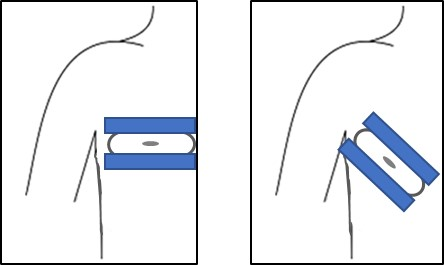
\includegraphics[width=0.5\textwidth,keepaspectratio]{figures/cc_mlo_view.jpg} 
\caption{left: cranio-caudal breast compression; righ: mediolateral oblique breast compression. }
\label{fig:cc_mlo_view}
\end{figure}

 The two views are complementary. The MLO view covers a large amount of tissue and provides a better visualization of the upper juxtathoracic part of the breast, while the CC-view suffers less from overlapping dense tissue and provides a better visualization on the central part of the breast \citep{chan_image_1987,kim_computer_2006}.  Further incidences or magnification views may be needed for diagnostic mammography \citep{groot_towards_2015}.
 

The mammography devices are equipped with paddle position and force sensors to measure and display the compressed breast thickness and the amount of force applied to the breast.

\section{Paddles designs} \label{section:compressionpaddlesdesign}

Nowadays, a wide range of compression paddles are available for breast clinical examination. Their shape and dimensions vary in function of the purpose for which they were designed but also from manufacturer to manufacturer. According to their specific
indications of use, three categories can be distinguished: \textbf{standard paddle} used for regular screening, \textbf{spot paddles} used for diagnosis purposes, and \textbf{biopsy paddles} used for breast compression during breast biopsy (Figure \ref{fig:compressionpaddlestypes}). 


\begin{figure}[!h]
\centering
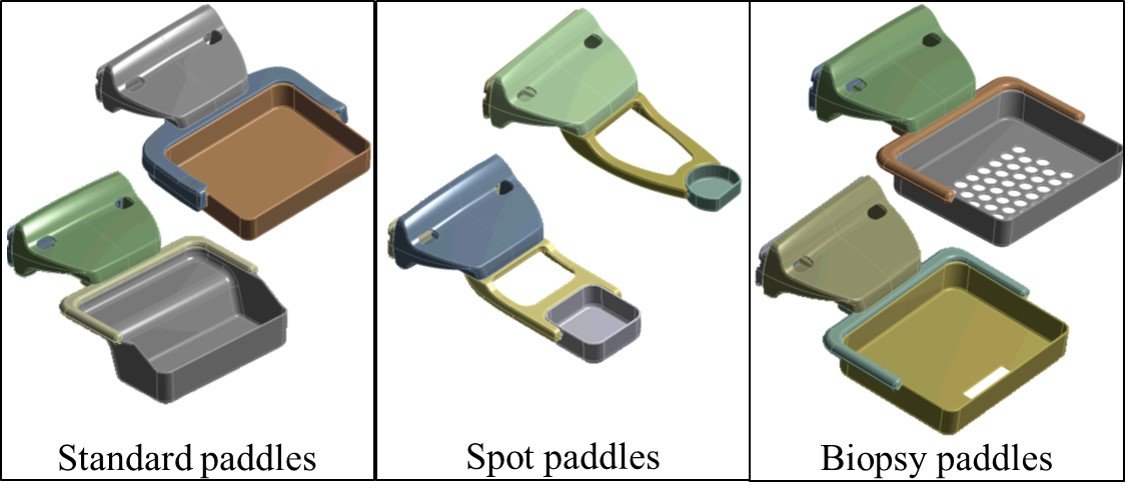
\includegraphics[width=0.9\textwidth,keepaspectratio]{figures/compressionpaddlestypes.jpg} 
\caption{Different breast compression paddles for GE Healthcare mammography units .}\label{fig:compressionpaddlestypes}
\end{figure}
    

 The standard compression paddles have usually a rectangular shape with a flat compression plate. Depending on the industrial manufacturer, they can have different sizes for both the lateral and longitudinal edges and for the paddle front edge height. Paddles with smaller compression area are used to compress small breasts or breasts with implants (Figure \ref{fig:compressionpaddlestypes}, Standard paddles). Standard paddles are classified into rigid and flexible paddles. The standard rigid paddle (SRP)\nomenclature{SRP}{ Standard Rigid Paddle} is fixed to its frame and is constrained to move in the up-down direction only. This paddle has some flexibility because of its material mechanical properties and can slightly bend when compressing the breast, while remaining globally parallel to the image receptor (Figure \ref{fig:compressionpaddles}.b). On the other hand, the standard flex paddle (SFP) \nomenclature{SFP}{Standard Flex Paddles} is attached to its frame by flexible joints and therefore, presents an additional degree of freedom enabling the paddle to tilt with respect to the image receptor plane (Figure 3.c). During compression the paddle remains parallel to the detector at first, tilts towards nipple side and then ends with the highest point at the thorax level. Depending on the breast position, the paddle may also slightly tilt in the medio-lateral direction.

\begin{figure}[!h]
\centering
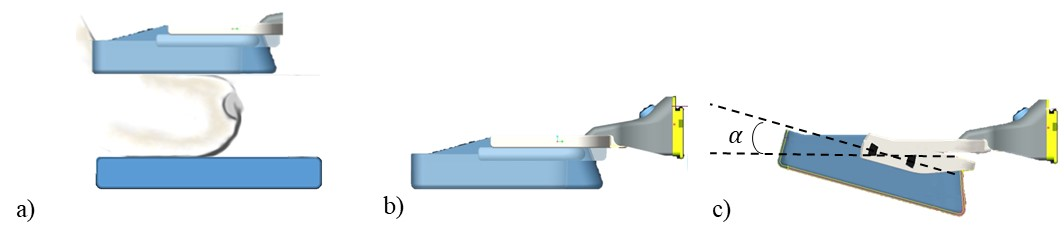
\includegraphics[width=0.9\textwidth,keepaspectratio]{figures/compressionpaddles.jpg} 
\caption{a) Breast compression between the paddle (up) and the image receptor (down): b) Rigid paddle; c)Flex paddle with a flexion angle $\alpha$}\label{fig:compressionpaddles}
\end{figure}


 Spot paddles apply the compression to a smaller area of tissue using a small compression plate or a cone. By applying compression to only a specific area of the breast, the effective pressure is increased on that spot. This results in a better tissue separation and allows for a better visualization of the small area in question.  It is used to distinguish between the presence of a true lesion and an overlap of tissues, as well as to better show the borders of an abnormality or questionable area or a little cluster of faint microcalcifications.  

Biopsy exams require that the patient's breast remain immobile and compressed during the entire procedure. The biopsy paddles have basically the same shape as the standard rigid paddles. However, to allow the needle insertion and the accessibility to the biopsied area, the paddle plate contains multiple holes with various diameter or a single aperture. 

In this chapter, only breast compression with the rigid paddle in the two main view (MLO and CC) is considered.

\section{Compression mechanics} \label{subsec:compressionmechanics}
Nowadays, the European Commission recommends a force standardized breast compression, i.e. a compression that stops at a level of force just below the subject's pain threshold or at the maximum force setting of the machine.  The compression guidelines state that force should be firm but tolerable with a maximum applied compression of 130-200 N \citep{perry_european_2008}. As there is no exact specification for the application of breast compression, the applied force may vary between technologists and radiologists. Mercer C. and colleagues \citep{mercer_practitioner_2013} have analyzed the variation of the applied force within 14 trained practitioners. Both views, CC and MLO, were included. The authors found a significant difference between the average applied forces and have highlighted three groups of radiologists depending on the mean force intensity. Between the consecutive groups, a mean difference of $16 \ N$ was found. 

The global breast compression cycle is characterized by two phases: flattening and clamping \citep{de_pain_2015}. During the flattening phase, the breast is gradually deformed by increasing the compression force; this step lasts about  $7.5 \pm 2.6\ s$. By contrast, during the clamping phase, which lasts approximately $12.8 \pm 3.6\ s$, the compression paddle is immobilized holding the breast in a stationary position. 
\begin{figure}[!h]
\centering
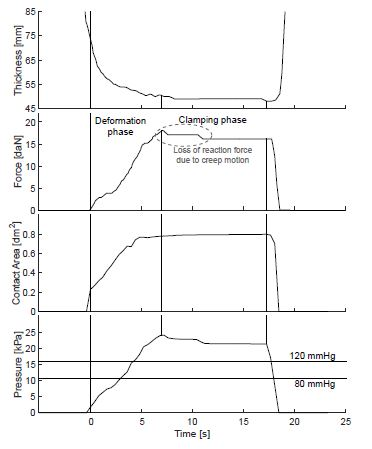
\includegraphics[width=0.7\textwidth,keepaspectratio]{figures/breast_compression_cycle.jpg} 
\caption{A typical breast compression cycle. Reproduced from Groot J.E. et al. \citep{groot_towards_2015}}\label{fig:breast_compression_cycle}
\end{figure}

Figure \ref{fig:breast_compression_cycle} shows a typical compression cycle for a CC breast compression from experimental data on real patients described by Groot J.E. et al. \citep{de_pain_2015}. One can see that, during compression phase, the breast thickness and contact area evolve non-linearly; meanwhile, the compression force and pressure increase quasi-linearly. During the clamping phase, the breast thickness remains constant; however, the skin pressure and the compression force slightly decreases in the first $10s$. This phenomenon may be explained by breast volume changes because of the viscous effusion of blood and lymph into the central systems. 

In the same work, the authors present several in-vivo measured patterns describing the relation between breast thickness and compression force depending on breast size and its firmness (Figure \ref{fig:thickness_force_patterns_groot}). One can see that, for a larger breast, higher compression force is needed but the overall behavior remains the same as for smaller breasts. For similar breast sizes, the final compression forces range within the same values, however a firmer breast will reach faster the limiting value of breast thickness resulting in an asymptotic increase of the compression force.
\begin{figure}[!h]
\centering
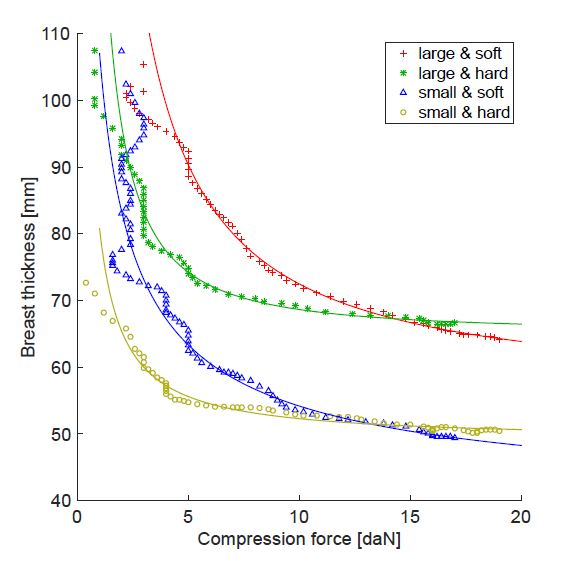
\includegraphics[width=0.6\textwidth,keepaspectratio]{figures/thickness_force_patterns_groot.jpg} 
\caption{In-vivo measured breast flattening curves as function of the applied force. Reproduced from Groot J.E. et al. \citep{groot_towards_2015}}\label{fig:thickness_force_patterns_groot}
\end{figure}

Dustler M. and colleagues \citep{dustler_breast_2012} have studied the pressure distribution patterns for MLO breast compression (55 degree tilt). The authors showed that the pressure distribution varies widely within the breast. The obtained patterns from 131 subjects were classified into four main groups: a) skin pressure widespread over the breast (29\%); b) skin pressure concentrated on the central part of the breast (8\%); c) skin pressure concentrated on the juxtathoracic region (16\%); d) skin pressure concentrated along a narrow zone at the juxtathoracic region (26\%). According to their results, the pressure distribution depends on two factors: the variation on breast thickness from one side and surrounding tissues stiffness from the other side. For example, for the groups c and d the breast anterior tissues compression is limited by the pectoral muscle which is much stiffer than the breast tissues.  These results may explain the fact that, in MLO view, the breast thickness exceeds the one on the CC view, despite the larger force used in MLO than in CC breast compression \citep{mercer_practitioner_2013, helvie_breast_1994}. 

\section{Compression quality metrics}
A standard mammography protocol always includes breast compression prior to image acquisition. The breast flattening improves diagnostic image quality and reduces the absorbed dose of ionizing photons. However, the discomfort and pain produced by this procedure sometimes might deter women from attending breast screening by mammography. 

An important improvement concerning the patient comfort could be achieved with the emergence of digital mammography. Indeed, several studies have shown that digital mammography is better in terms of image quality \citep{obenauer_screen_2002} and radiation dose \citep{chen_analysis_2012} than film-screen mammography.

Most digital mammography systems have an automatic beam quality selection mode (automatic optimization of parameters, AOP\nomenclature{AOP}{Automatic Optimization of Parameters}) with an automatic exposure control (AEC \nomenclature{AEC}{Automatic Exposure Control}). The AOP mode automatically selects the X-ray  tube  voltage, the anode  target  material  and  filter  material defining the X-ray spectrum, in order to optimize the \textit{contrast to dose ratio}, i.e. the appropriate amount of radiation for an acceptable low dose and an increased contrast, according to breast thickness and composition \citep{williams_optimization_2008}. Then, the required exposure time for the actual image is calculated by the AEC.  The AOP control allows to determine, for each patient and compression level, the X-ray spectrum that optimizes the  ratio of benefits  (higher image contrast) and  drawbacks  (higher  dose). 
In this section, the compression quality will be measured in terms of three metrics: image quality, average dose and patient comfort. A detailed description of each metric is given below with their impact for digital mammography. 

\subsection{Image quality}

Many factors may influence the quality of the mammography image such as the knowledge and skill of the person who performs the mammography examination, the equipment, the positioning
technique, and the compressed breast thickness, type of breast
cancer, and radiographic appearance of the breast tissue \citep{de_pain_2015,andolina2011mammographic}. In our study, only the impact of the compressed breast thickness on image quality is analyzed.

 Firstly, the breast compression facilitates the image interpretation. Higher compression leads to better tissues spread and consequently to less overlapping of clinical important structures. A thinner layer of breast tissues allows a more subtle differentiation between normal and suspicious findings. Secondly, breast compression affects the image sharpness. Since the exposure time lasts several seconds, a proper breast immobilization reduces the image blurring, preserving the conspicuity of abnormal legions. Moreover, with a reduced breast thickness, the primary contrast is raised due to the reduction of radiation scatter to primary ratio at detector level. Finally, the breast compression leads to a better use of the detector dynamic range. With a non-uniform breast thickness, the different levels of brightness are used to describe the thickness variation, thus the detector dynamic is not used optimally for the contrast representation due to different internal structures. This is particular true for screen-film technology, with digital detectors; this constraint can be challenged.

It has been proved that image quality decreases with increasing breast thickness \citep{ko_dose_2013,helvie_breast_1994,saunders_effect_2008,poulos_breast_2003}. Helvie M. and colleagues \citep{helvie_breast_1994} analyzed the image quality for the observed breast thickness of 250 subjects using film-screen mammography.  The difference in breast thickness and image quality between the MLO and CC paired images were computed. According to the authors, image sharpness decreased by 19\% for $1\ cm$ of increased breast thickness. In addition, contrast loss was observed due to scatter augmentation and beam hardening.

Later, Saunders R.S. et al. \citep{saunders_effect_2008} have studied the effect of breast compression on mass conspicuity in digital mammography using Monte Carlo based simulation framework. The simulation was done for two breast thicknesses $(4\ cm\ and\ 6\ cm)$ with two compression levels (standard and reduced compression by $12\%$) and three photon flux conditions (constant
flux, constant detector signal, and constant glandular dose). The results suggest that if a particular imaging system can handle an approximately 10\% increase in total tube output and 10\% decrease in detector signal, breast compression can be reduced by about 12\% in terms of breast thickness with little impact on image quality or dose.

O'Leary D. et al. \cite{oleary_compression_2011} performed a clinical study to assess the image quality in function of the applied compression force for digital mammography. The CC and MLO views of 4790 subjects were analyzed and image quality was categorized as  perfect, good, moderate or
inadequate. The results have shown that the image quality is highly correlated with the applied force. The mean compression force required to produce a perfect image was found to be equal to 121.34 N for a CC view and 134.23 N for a MLO view.

\subsection{Average glandular dose}
A mammography unit uses X-rays to obtain 2D-projection images from the breast tissues. As for any X-ray exposure, the irradiation of a targeted population is accepted if the benefits are significantly higher than the risks. Therefore,  mammography exposures must provide a good image quality while preserving the radiation dose \textit{as low as reasonably achievable}.

To assess the quality of breast compression, the risk from the X-ray exposure have to be considered.  The absorbed energy from digital mammography depends on many factors such as the breast density, the breast thickness, the volumetric distribution of glandular tissues as well as the acquisition parameters. 

It has been proved that glandular tissues of the breast are more vulnerable to radiation carcinogenesis than skin, adipose tissue, or areola \citep{richard_absorbed_1979}. Based on these findings, the average glandular dose (AGD) was defined to quantify the risk from breast irradiation and is widely accepted for regulations.  The most often used method calculates the AGD as the product of the incident air kerma\footnote{radiation dose measurement at a point on a patient's skin} at the upper surface of the breast with conversion factors called \textit{normalized dose}. The normalized dose (DgN) \nomenclature{DgN}{Normalized dose} is computed as a function of spectrum, breast thickness and breast density.  Its computation is based on Monte Carlo simulations \citep{dance_additional_2000,boone_glandular_1999}. 

Historically, only rigid paddles were used for breast cancer screening. Therefore, in numerical simulations, the breast is usually modeled as a flat semicircular object with a homogeneous content and surrounded by a layer of skin. The attenuation coefficient of the content corresponds to the breast density, the ratio of the amount of gland to total breast \citep{dance_additional_2000}.

 When a flex paddle is used, the breast thickness decreases towards the nipple side, resulting in a wedge-shaped breast.  Since the AGD model assumes a flat shape, apart from inherent uncertainties due to general assumptions concerning breast geometry and composition, additional uncertainties due to the paddle tilt are included. In a clinical framework, no difference is made between the flex and the rigid paddles for the AGD computation \citep{broeders_comparison_2015}. To our knowledge, the associated errors are not quantitatively described in the literature.  

Recent reports have updated dose estimates from screen-film mammography (SFM\nomenclature{SFM}{Screen-Film Mammography}) and full field digital mammography, indicating that two-view screening with FFDM delivers a slightly lower dose than does SFM . The mean average dose was estimated for different populations. A geographical classification shows that the AGD delivered by digital mammography for a European woman  $(1.48 mGy)$ is higher on average than the one for North American $(1.42 mGy)$ or Asian woman $(1.42 mGy)$ \citep{geeraert_breast_2012}. Osteras B. and colleagues \cite{osteraas_average_2018} have classified the CC and MLO view of 3819 women in two classes by breast density. The authors reported a mean AGD of $1.73 mGy$ for the dense breasts and an AGD of $1.74 mGy$ for the fatty breasts. The AGD was estimated using the model proposed by Dance D. et al. \cite{dance_additional_2000} .  


\subsection{Pain and discomfort}
Many women have reported discomfort or pain during mammography exams. A literature review over the last decades shows that the  prevalence of pain varies widely, the percentage of women experiencing pain or discomfort ranging between 16\% and 72\% \citep{keemers_pain_2000, peipins_impact_2006,dullum_rates_2000, whelehan_effect_2013}. This difference could be due to the interpretation of pain intensity (i.e. distinction between \textit{pain} and \textit{considerable pain}),  but also could be attributed to differences in the instruments used to measure pain. 

Pain intensity is influenced by the meaning of the pain to the patient and its expected duration. The environment also has an impact on the experience of pain, as do expectations, attitudes and beliefs. Pain is rarely caused by psychological factors, but is associated with psychological and emotional effects such as fear, anxiety and
depression \citep{williamson_pain_2005}.

The three most-used pain metrics in clinical studies are the visual analogue scales, the numeric rating scales and the verbal rating scale \citep{williamson_pain_2005}. The \textbf{visual analogue scale} (VAS)\nomenclature{VAS}{Visual Analogue Scale} is presented as 10-cm continuous line together with a verbal descriptors at the line's ends (no pain and worst imaginable pain). The patient is asked to mark the pain intensity on the line. The score is measured from the zero to the patient's mark using a millimeter scale which provide 101 levels of pain intensity. The \textbf{numerical rating scale} (NRS)\nomenclature{NRS}{Numerical Rating Scale} is a discrete point scale were the end points are the extremes of the pain range. In mammography, a 6 or 11 point scale is generally used.  The patient will mark the point corresponding to the perceived pain intensity. The \textbf{verbal rating scale} (VRS)\nomenclature{VRS}{Verbal Rating Scale} comprises a list of adjectives used to denote increasing pain intensities, such as no pain, mild pain, moderate pain and severe pain. The patient will choose the adjective corresponding to the perceived pain intensity. According to Williams M. et al. \citep{williamson_pain_2005} the numerical rating scale provides the best trade-off between metric sensitivity and the metric repeatability.     

In mammography, the pain experienced by women during the exam depends on psychological (technician behavior, patient anxiety) \citep{aro_pain_1996}, sociological  (ethnicity, education level) \citep{dullum_rates_2000} and physiological factors (compression level, breast size)\citep{poulos_breast_2003}.  It was found that, the main factors associated with the patient discomfort are the satisfaction with care and the perception of the technologist's \textit{roughness} \cite{dullum_rates_2000}. Besides this findings, several studies have also suggested the pain expectation and the anxiety level as ones of the main risk factors associated with the pain \citep{aro_pain_1996,williamson_pain_2005,keemers_pain_2000,askhar_female_2017}.   

The physiological factors such as breast thickness, breast size or periods are also positively correlated with the patient comfort \citep{keemers_pain_2000,hafslund_mammography_2000}. The relationship between applied compression force, breast thickness, reported discomfort and image quality has been studied by Poulos A. et al \citep{poulos_breast_2003}. According to the authors, the patient comfort decrease with the compressed breast thickness. The authors reported a significant relationship between patient discomfort and breast thickness. However, no significant relationship between the reported discomfort of the procedure and the applied compression force was found. According to the authors, force does not correlate well with subject discomfort since it does not account for differences in breast thickness.
 
A painful mammography contributes to non-re-attendance. Twenty five percents of US women rated their experience of screening 30
months after their latest mammogram as at least moderately painful \cite{peipins_impact_2006}. It is thus plausible that remembered pain can possibly dissuade women from
attending later screening exams.

\section{Recent advances in breast compression}\label{section:compressionrecentadvances}

Breast compression is an important part of mammography exams. A good breast compression improves image quality, better separates breast tissues structures and reduces the absorbed dose. In the same time, breast positioning and compression are the main sources of discomfort experienced by patients. Because anxiety is documented to be the most important contributor to procedural pain, interventions designed to reduce both physical and psychologic discomfort are needed.


Considering the previous listed risk factors, various pain reducing techniques concerning the usual care were proposed during the last years \citep{miller_interventions_2008}. To decrease the patient anxiousness and pain expectations, verbal and written information was proposed prior to mammogram. Informing the patients and accompanying them during the exam have shown to decrease the population mean pain score from 25 to 17 in a 100-mm VAS \citep{shrestha_effect_2001}. In the same time, the effect of some relaxation techniques has been studied. Domar A. et al. \cite{ domar_relaxation_2005} compared the perceived pain from an usual mammogram to the one  accompanied by music or a relaxation audiotape. The music subjects had a choice of classical music, jazz, or soft rock.  The relaxation audiotape contained information that led the subject through breath focus, body scan, and meditation. According to the authors, there was no significant difference in perceived pain between the various groups. 

Later, with the emergence of digital mammography, pain reducing compression techniques were proposed. Several studies \citep{chida_reduced_2009,saunders_effect_2008} suggest that the compression force may be reduced by at least 10\% without a significant impact on image quality or average glandular dose. However, according to Poulos A. et al. \cite{poulos_breast_2003}, the patient comfort is not related to the applied force intensity but to the compressed breast thickness, which in its turn is associated with the breast size and firmness. To achieve the optimal compression considering the patient breast specific morphology, a pressure controlled compression is recommennded instead of a force controlled compression \citep{de_pain_2015}. The recommended target pressure is equal to $10\ kPa$. For a clinical integration, the SegmaScreening company has proposed a new standard rigid paddle with integrated pressure control while the Volpara Solutions company has proposed a software computing the contact area between the breast and the compression paddle in order to extrapolate the mean applied pressure.  In the same time, Dustler M. et al \cite{dustler_effect_2012} analyzed alternative breast positioning according to previously found pressure distribution patterns. Because of stiff juxtathoracic structures, the authors proposed to increase the distance between the compression paddle and the chest wall by 1cm. The results have shown that within the new breast positioning, the pressure is reduced on the juxtathoracic area. The breast thickness was decreased by $4.4\pm2.3 \ mm$ with no significant effect on force intensity. However, the six participants have identified the repositioned compression as the most painful, which, according to the authors, may be explained by the higher pressure intensities on the overall breast surface itself.  The main drawback of this technique is the exclusion of juxtathoracic tissues which may obscure small posterior suspicious legions. 
 
According to latter studies, several constructors started to propose various solutions to reduce the physical discomfort during mammography. Hologic company proposed the MammoPad cushion which is claimed to reduce the discomfort by 50\%. In the review proposed by \cite{miller_interventions_2008}, such radiolucent breast cushions are supposed to reduce the pain score (100mm VAS) from 35 to 20 in CC view and from 43 to 26 in MLO. GE Healthcare company proposed a patient-controlled breast compression with the new Senographe Pristina system. This technique lets women controling them selves how much the device compresses their breasts.  The breast is firstly positioned by the technologist between the compression plates; then, the patient is terminating her compression up to a level she can support. It has been shown that the patient-controlled compression is less painful than the techologist-controlled compression with no significant impact on image quality  \citep{miller_interventions_2008}.

The breast positioning is a fastidious task for the technologist. For example, a larger amount of posterior tissue included in breast compression may result in a thicker breast at the anterior area, which in its turn may reduce the image quality and hide important clinical information. The technologist has the critical job of applying positioning methods using common sense. If the breast area is not well covered by the first two projections, an additional third projection may be necessary. The use of flex paddles proposed by some constructors, such as American Mammographics S.O.F.T. Paddle, GE Healthcare Flex Paddle or Hologic FAST Paddle aims at increasing the area of compressed tissues and thus avoiding an additional projection.

To our knowledge, there is only one study assessing the difference in image quality, average glandular dose and patient comfort between flex and rigid paddles \citep{broeders_comparison_2015}. According to the authors the flex paddle affects the technical image quality without improving the patient experience.  Because the flex paddle pulls the soft tissues towards the pectoral wall, they are less visible in the image. It must be highlighted that the study of Broeders and colleagues included CC and MLO projections with force-controlled compressions (target force between 12-20 daN). Based on the same principle as the study presented by Dustler M. et al \cite{dustler_effect_2012}, one may guess that breast compression with a flex paddle will result in a higher pressure over the breast surface itself (less pressure on the juxtathoracic area which may be the origin of the pain over the breast surface). It may be interesting to assess the patient discomfort and the image quality with a pressure-controlled compression. Moreover, the average glandular dose is computed by neglecting the wedge form of the flex paddle, therefore it is difficult to compare the flex and the rigid paddles.  

To better quantify the difference between flex and rigid paddles, further investigations are needed.  In this scope, we have developed a simulation framework allowing to assess breast compression quality in function of breast patient specific morphology and compression paddle design.\\
\\


This framework is presented in the next chapter, where the breast compression modeling by finite element as well as the numerical methods to assess the corresponding image quality and the average glandular dose are described. In a numerical environment, it is almost impossible to model the psychological patient discomfort, thus this work is focused on analyzing the patient physical discomfort which here is assumed to be associated with tissues internal strain/stress due to breast compression. Ultimately, the breast compression quality for CC view is evaluated for flex and rigid paddles and for various paddle positions.
